\subsection{SDMetrics}
\sdmetrics\ is a design measurement tool for analyze a wide range of \uml\ diagrams, including Class, Use Case, Activity and Statemachine diagrams.

For each type of diagram, this tool generates several metrics.
For example, the \textbf{NumAttr} metric is calculated from Class diagrams and measures the number of attributes in a class.
Other one is \textbf{ExtPts}, which is calculated from Use Case diagrams, and gives us the number of extension points of a given use case.

\sdmetrics\ is written in \textsf{Java}, and provides us a graphical user interface for analyze \xmi\footnote{
\xmi\ (\textbf{X}ML \textbf{M}etadata \textbf{I}nterchange)  is an \emph{OMG} (Object Management Group) standard to generate \xml-based representations of \uml\ and other OO data models.} 
files, most modeling tools support project exportation in \xmi.

This tool allows to access the results from different views. We will introduce the ones that seem the most important:
\begin{itemize}

\item \textbf{Metric Data Tables} provides a table that matches each \uml\ model element analyzed (table line) to its value for each metric (table column);
\item \textbf{Histograms} provides a graphical distribution  for each design metric;
\item \textbf{Design Comparison} provides us a mean to compare the structural properties of two \uml\ designs. It is very useful to compare the same design in different iterations of the development, or to compare an alternative design to the current one.
\item \textbf{Rule Checker} design rules and heuristics detect potential problems in the \uml\ design such as incomplete design (i.e. unnamed classes, states without transitions, etc.);  violation of naming conventions for classes, attributes, operations, packages; etc;

\begin{comment}
	\begin{itemize}
	\item incomplete design such as unnamed classes, states without transitions;
	\item violation of naming conventions for classes, attributes, operations, packages;
	\item etc.
	\end{itemize}
\end{comment}

\item \textbf{Catalog} this view provides us with the definitions of the metrics, design rules, and relation matrices for the current data set, and provides literature references and a glossary for them.
\end{itemize}

One of the most advanced features in this software is the possibility of defining Custom Design Metrics and Rules. 
The new metrics are defined in a \xml file, with a very particular format, the \emph{SDMetricsML} (\sdmetrics Markup Language).

The \sdmetrics\ tool does not provide a direct notion of good or bad quality of the design model. 
Despite that, on its User Manual\footnote{\url{http://www.sdmetrics.com/manual/index.html}} we can find tips of how to interpret each kind of metrics. 
 
\subsubsection{Results}
Based on the \sdmetrics\ manual, we will now explain how to analyze each metric obtained. 
Figure~\ref{fig:sdmetrics} illustrates some outputs of \sdmetrics\ for our case-study. 
On the left, we can see an Histogram for class diagrams evaluating the \emph{NumAttr} metric. On the right, we present an excerpt of a general metrics table for class diagrams.
%Next we will show some printscreen taken from SDMetrics, which will illustrate some of the outputs of this software, for our case-study.\\

\begin{figure}[htbp]
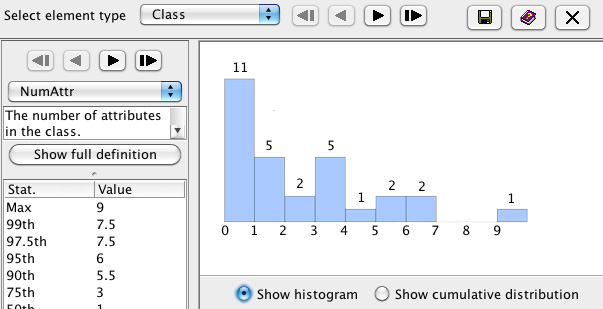
\includegraphics[scale=0.3]{images/histogram2}
\hspace{0.1cm}
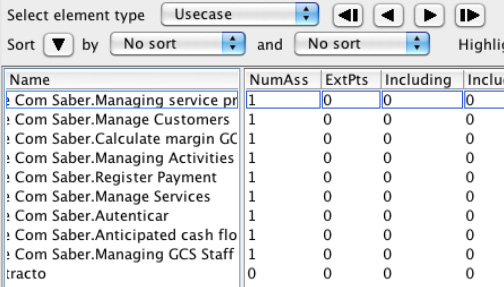
\includegraphics[scale=0.32]{images/table3}
\caption{\sdmetrics: \textsf{NumAttr} Histogram and Metrics Table for Use Case Diagrams}
\label{fig:sdmetrics}
\end{figure}


\begin{comment}
\textbf{Metrics Table}
\begin{figure}[H]
\begin{center}
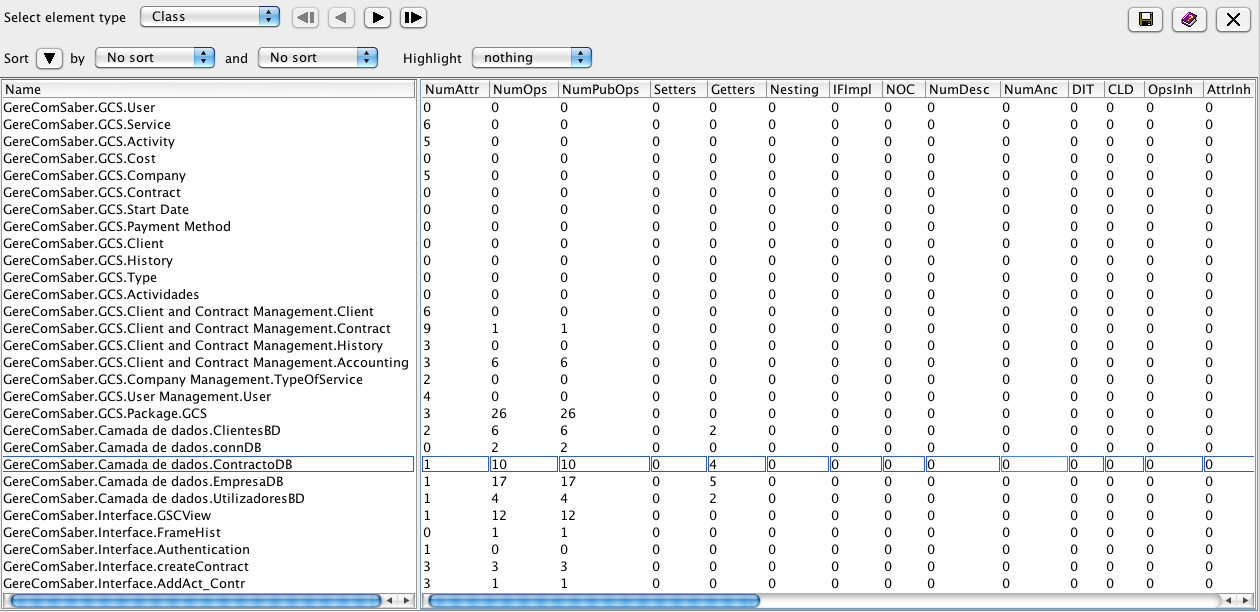
\includegraphics[width=1\textwidth]{images/table.png}
\caption{Metrics Table for class diagrams}\label{img:table}
\end{center}
\end{figure} 

\textbf{Histogram}
\begin{figure}[H]
\begin{center}
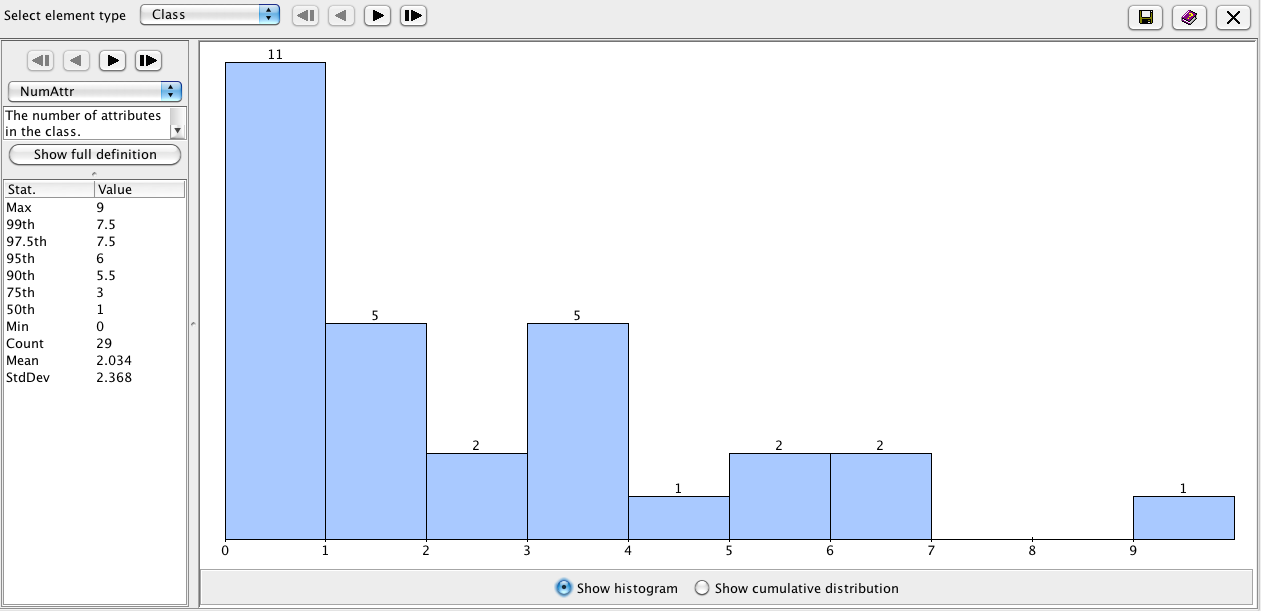
\includegraphics[width=1\textwidth]{images/histogram.png}
\caption{Histogram for class diagrams evaluating the metric NumAttr}\label{img:histogram}
\end{center}
\end{figure} 

\textbf{Rule Checker}
\begin{figure}[H]
\begin{center}
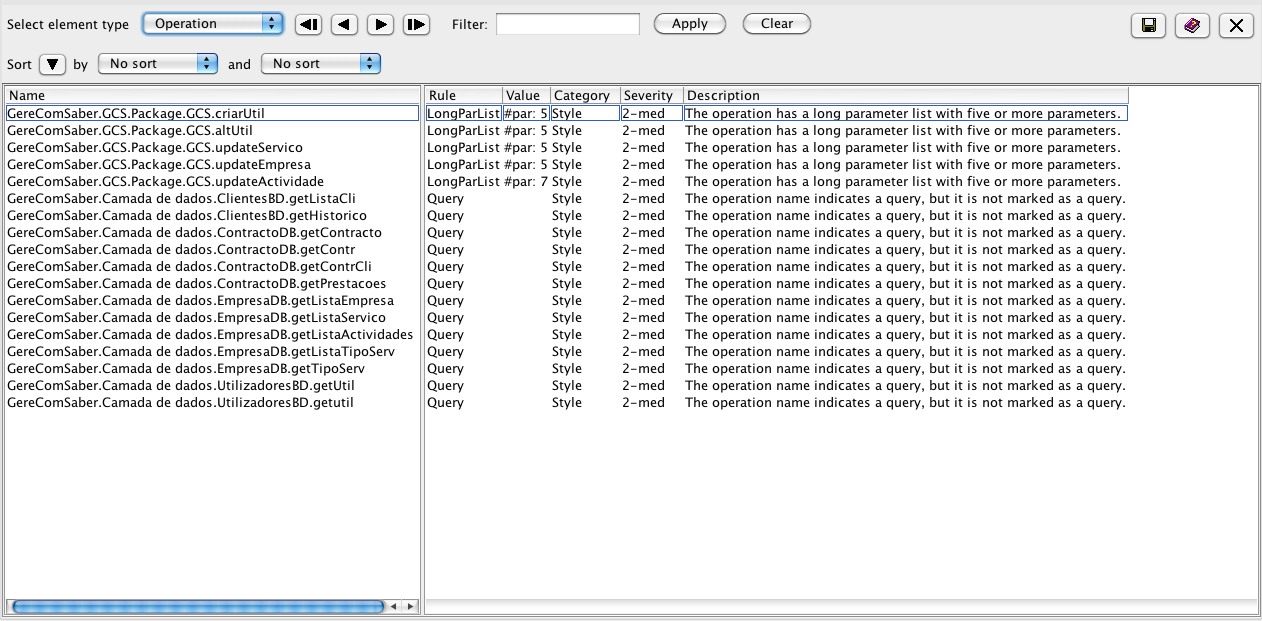
\includegraphics[width=1\textwidth]{images/rule.png}
\caption{Rule checking for Operations}\label{img:rule}
\end{center}
\end{figure} 
\end{comment}



Size metrics, which usually count elements inside design elements (class, package, etc), are good to estimate developing costs and effort, and can be directly found on the Metrics Table.
A large design element may indicate that it suffers from poor design, resulting in low functional cohesion. This has a negative impact on the understandability, reusability, and maintainability of the design element.

%The coupling between design elements is also measured by \sdmetrics. 
Coupling is the degree to which the elements in a design are connected: the more they are connected, the more they depend on each others. This high degree of dependency may affect the system maintainability, because when you change a design element, you may need to adapt the connected elements; and the system testability, because a problem in a design element may cause failure in a completely different connected element. Taking this in consideration, it is important to minimize coupling.

Inheritance-related metrics usually calculate features such as depth/width of the inheritance and number of ancestors/descendents of a design element. Such as high coupled elements, deep inheritance structures are believed to be more fault-prone. It is harder to fully understand a class that is situated deep in the inheritance tree, because you have to understand its ancestors. Also, modifying a design element with many descendants, may have a large impact on the system.

Complexity metrics measure the degree of connectivity between elements of a design element. They are concerned with relationships/dependencies between the elements in the design unit, such as the number of method invocations inside a class. The high complexity between the elements of a design element can make the design harder to understand, therefore more propitious to faults. Complexity metrics are usually strongly correlated with size measures. So even though they are good indicators of quality, such as fault-proneness, they provide no new knowledge comparing to size metrics.\\

In general, this directions lead us to beliefe that the lower the metrics values are, the better. Looking at the modelation which is our case study, it is not easy to establish  a maximum value for each metric. Either way, and looking at the modelation as an all, \textit{GCS} class for examle, seems to have to many operations (26), specialy compared to the rest of the classes. On the other hand, some classes look like they are missing operations. Taking this in regard, we should analyse carefully this classe, and perceive which operations do not belong to it, and should be given to other classes. Also classes that lack operations, should be completed.

This is just an example of how the output of \sdmetrics\ could be usefull during the modelation process.
